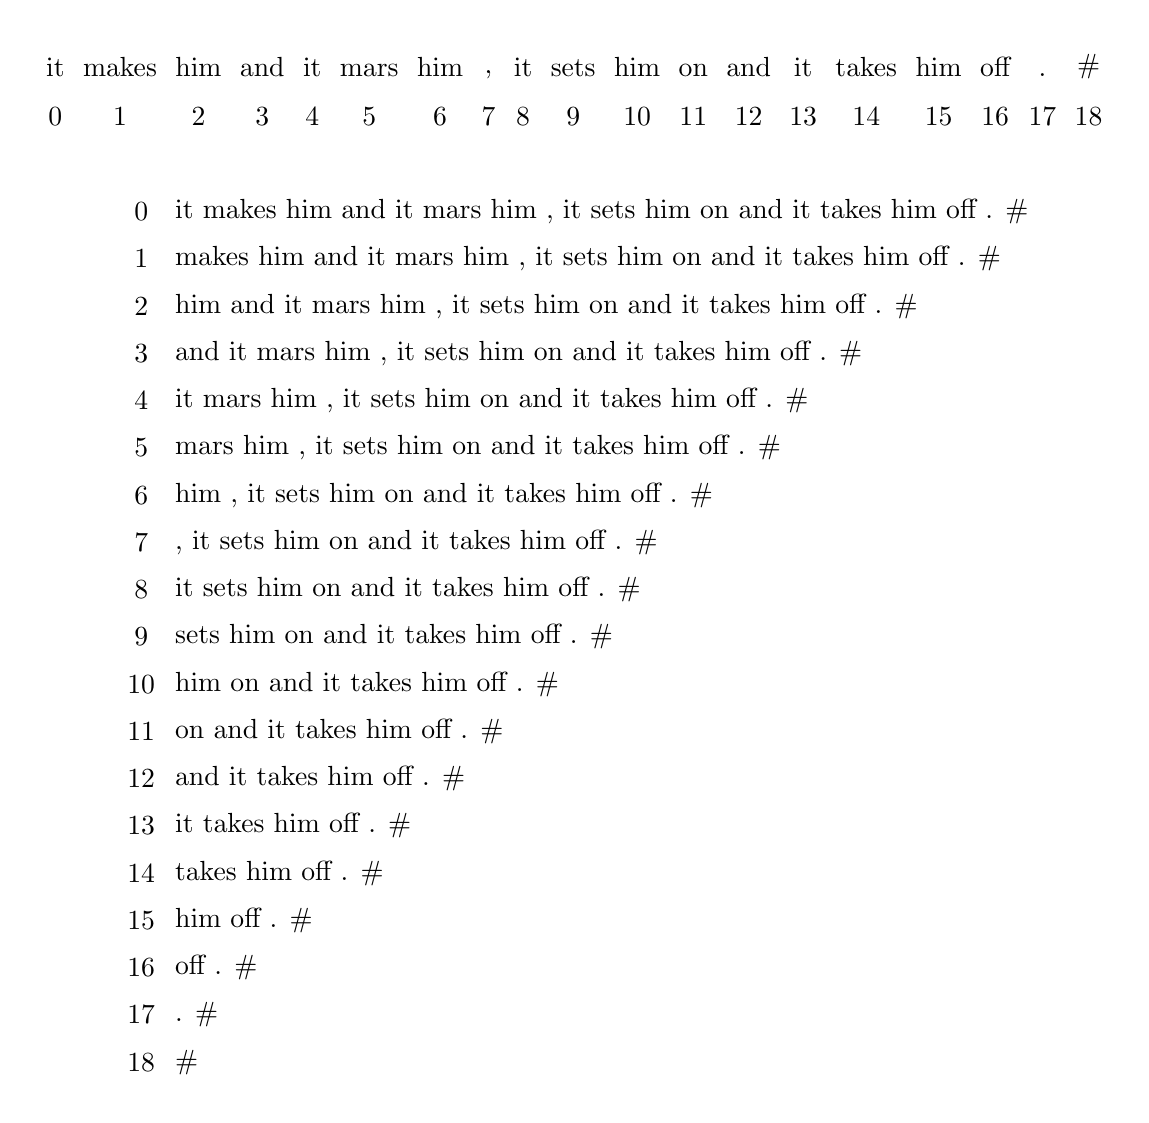
\begin{tikzpicture}
	\matrix (sentence) [nodes={text height=10pt}] at (5.5,7){
	\node {it}; & \node(word){makes}; & \node{him}; & \node{and}; & \node{it}; & \node{mars}; & \node {him}; & \node{,}; & \node{it}; & \node{sets}; & \node{him}; & \node{on}; & \node{and}; & \node{it}; & \node{takes}; & \node{him}; & \node{off}; & \node{.}; & \node{\#};\\
	\node {0}; & \node(num){1}; & \node{2}; & \node{3}; & \node{4}; & \node{5}; & \node {6}; & \node{7}; & \node{8}; & \node{9}; & \node{10}; & \node{11}; & \node{12}; & \node{13}; & \node{14}; & \node{15}; & \node{16}; & \node{17}; & \node{18};\\
	};

	\matrix [nodes={rectangle,minimum size=6mm}] at (0,0){
		\node (suffix 0) {0}; \\
		\node (suffix 1) {1}; \\
		\node (suffix 2) {2}; \\
		\node (suffix 3) {3}; \\
		\node (suffix 4) {4}; \\
		\node (suffix 5) {5}; \\
		\node (suffix 6) {6}; \\
		\node (suffix 7) {7}; \\
		\node (suffix 8) {8}; \\
		\node (suffix 9) {9}; \\
		\node (suffix 10) {10}; \\
		\node (suffix 11) {11}; \\
		\node (suffix 12) {12}; \\
		\node (suffix 13) {13}; \\
		\node (suffix 14) {14}; \\
		\node (suffix 15) {15}; \\
		\node (suffix 16) {16}; \\
		\node (suffix 17) {17}; \\
		\node (suffix 18) {18}; \\
	};
	\node [anchor=west] at (suffix 0.east) {it makes him and it mars him , it sets him on and it takes him off . \#};
	\node [anchor=west] at (suffix 1.east) {makes him and it mars him , it sets him on and it takes him off . \#};
	\node [anchor=west] at (suffix 2.east) {him and it mars him , it sets him on and it takes him off . \#};
	\node [anchor=west] at (suffix 3.east) {and it mars him , it sets him on and it takes him off . \#};
	\node [anchor=west] at (suffix 4.east) {it mars him , it sets him on and it takes him off . \#};
	\node [anchor=west] at (suffix 5.east) {mars him , it sets him on and it takes him off . \#};
	\node [anchor=west] at (suffix 6.east) {him , it sets him on and it takes him off . \#};
	\node [anchor=west] at (suffix 7.east) {, it sets him on and it takes him off . \#};
	\node [anchor=west] at (suffix 8.east) {it sets him on and it takes him off . \#};
	\node [anchor=west] at (suffix 9.east) {sets him on and it takes him off . \#};
	\node [anchor=west] at (suffix 10.east) {him on and it takes him off . \#};
	\node [anchor=west] at (suffix 11.east) {on and it takes him off . \#};
	\node [anchor=west] at (suffix 12.east) {and it takes him off . \#};
	\node [anchor=west] at (suffix 13.east) {it takes him off . \#};
	\node [anchor=west] at (suffix 14.east) {takes him off . \#};
	\node [anchor=west] at (suffix 15.east) {him off . \#};
	\node [anchor=west] at (suffix 16.east) {off . \#};
	\node [anchor=west] at (suffix 17.east) {. \#};
	\node [anchor=west] at (suffix 18.east) {\#};

\end{tikzpicture}
